\begin{figure*}
    \centering
    \vspace*{-0.25cm}
    \begin{subfigure}[t]{0.02\textwidth}
        \vspace{0px}
        \rotatebox{90}{\small\clean\hspace*{0.25cm}}
    \end{subfigure}
    \begin{subfigure}[t]{0.1\textwidth}
        \vspace{0px}
        \centering
        \small Input\\
        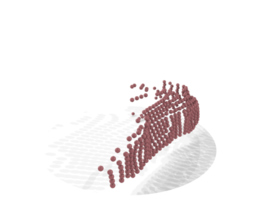
\includegraphics[width=1.75cm,trim={0.5cm 0.75cm 1.5cm 1.5cm},clip]{gfx/experiments_data/clean*/points/00002}
    \end{subfigure}
    \begin{subfigure}[t]{0.1\textwidth}
        \vspace{0px}
        \centering
        \small\ML\\
        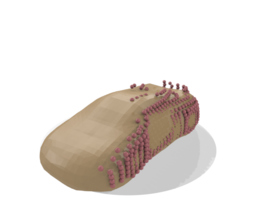
\includegraphics[width=1.75cm,trim={0.5cm 0.75cm 1.5cm 1.5cm},clip]{gfx/experiments_shapenet_kitti/vae_occ+sdf_ml/sb.clean.10.large.const15*/sdf_points/00002}
    \end{subfigure}
    \begin{subfigure}[t]{0.1\textwidth}
        \vspace{0px}
        \centering
        \small\cite{Engelmann2016GCPR}\\
        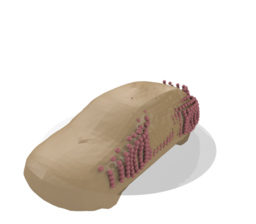
\includegraphics[width=1.75cm,trim={0.5cm 0.75cm 1.5cm 1.5cm},clip]{gfx/experiments_shapenet_kitti/engelmann2016/clean*/sdf_points/00002}
    \end{subfigure}
    \begin{subfigure}[t]{0.1\textwidth}
        \vspace{0px}
        \centering
        \small\AML\\
        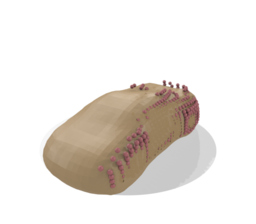
\includegraphics[width=1.75cm,trim={0.5cm 0.75cm 1.5cm 1.5cm},clip]{gfx/experiments_shapenet_kitti/vae_occ+sdf_aml/sb.clean.10.large.const15*/sdf_points/00002}
    \end{subfigure}
    \begin{subfigure}[t]{0.1\textwidth}
        \vspace{0px}
        \centering
        \small\AML\\
        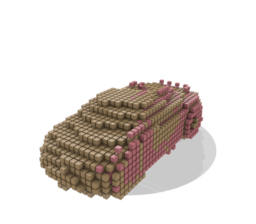
\includegraphics[width=1.75cm,trim={0.5cm 0.75cm 1.5cm 1.5cm},clip]{gfx/experiments_shapenet_kitti/vae_occ+sdf_aml/sb.clean.10.large.const15/binvox_points/00002}
    \end{subfigure}
    \begin{subfigure}[t]{0.1\textwidth}
        \vspace{0px}
        \centering
        \small\Sup\\
        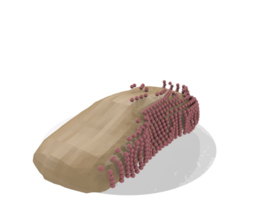
\includegraphics[width=1.75cm,trim={0.5cm 0.75cm 1.5cm 1.5cm},clip]{gfx/experiments_shapenet_kitti/vae_occ+sdf_sup/sb.clean.10.large*/sdf_points/00002}
    \end{subfigure}
    \begin{subfigure}[t]{0.1\textwidth}
        \vspace{0px}
        \centering
        \small\Sup\\
        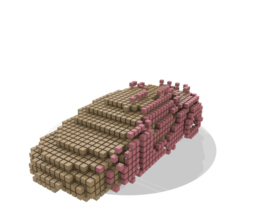
\includegraphics[width=1.75cm,trim={0.5cm 0.75cm 1.5cm 1.5cm},clip]{gfx/experiments_shapenet_kitti/vae_occ+sdf_sup/sb.clean.10.large/binvox_points/00002}
    \end{subfigure}
    \begin{subfigure}[t]{0.1\textwidth}
        \vspace{0px}
        \centering
        \small GT\\
        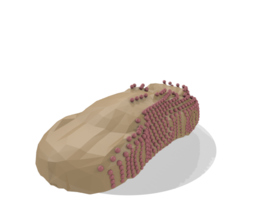
\includegraphics[width=1.75cm,trim={0.5cm 0.75cm 1.5cm 1.5cm},clip]{gfx/experiments_data/clean*/simplified/00002}
    \end{subfigure}
    \begin{subfigure}[t]{0.1\textwidth}
        \vspace{0px}
        \centering
        \small GT\\
        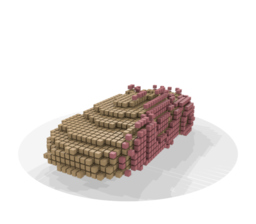
\includegraphics[width=1.75cm,trim={0.5cm 0.75cm 1.5cm 1.5cm},clip]{gfx/experiments_data/clean/voxelized/00002}
    \end{subfigure}\\
    % -------------------------------------------------------------------------------------------------
    % -------------------------------------------------------------------------------------------------
    \begin{subfigure}[t]{0.02\textwidth}
        \vspace{0px}
        \rotatebox{90}{\small\clean\hspace*{0.25cm}}
    \end{subfigure}
    \begin{subfigure}[t]{0.1\textwidth}
        \vspace{0px}
        \centering
        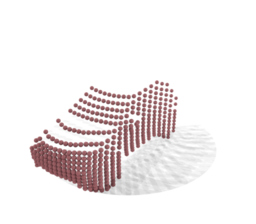
\includegraphics[width=1.75cm,trim={0.5cm 0.75cm 1.5cm 1.5cm},clip]{gfx/experiments_data/clean*/points/00007}
    \end{subfigure}
    \begin{subfigure}[t]{0.1\textwidth}
        \vspace{0px}
        \centering
        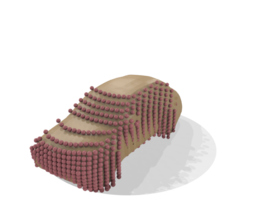
\includegraphics[width=1.75cm,trim={0.5cm 0.75cm 1.5cm 1.5cm},clip]{gfx/experiments_shapenet_kitti/vae_occ+sdf_ml/sb.clean.10.large.const15*/sdf_points/00007}
    \end{subfigure}
    \begin{subfigure}[t]{0.1\textwidth}
        \vspace{0px}
        \centering
        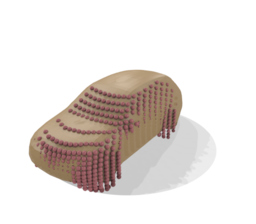
\includegraphics[width=1.75cm,trim={0.5cm 0.75cm 1.5cm 1.5cm},clip]{gfx/experiments_shapenet_kitti/engelmann2016/clean*/sdf_points/00007}
    \end{subfigure}
    \begin{subfigure}[t]{0.1\textwidth}
        \vspace{0px}
        \centering
        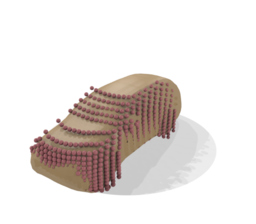
\includegraphics[width=1.75cm,trim={0.5cm 0.75cm 1.5cm 1.5cm},clip]{gfx/experiments_shapenet_kitti/vae_occ+sdf_aml/sb.clean.10.large.const15*/sdf_points/00007}
    \end{subfigure}
    \begin{subfigure}[t]{0.1\textwidth}
        \vspace{0px}
        \centering
        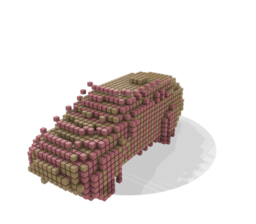
\includegraphics[width=1.75cm,trim={0.5cm 0.75cm 1.5cm 1.5cm},clip]{gfx/experiments_shapenet_kitti/vae_occ+sdf_aml/sb.clean.10.large.const15/binvox_points/00007}
    \end{subfigure}
    \begin{subfigure}[t]{0.1\textwidth}
        \vspace{0px}
        \centering
        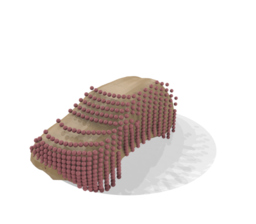
\includegraphics[width=1.75cm,trim={0.5cm 0.75cm 1.5cm 1.5cm},clip]{gfx/experiments_shapenet_kitti/vae_occ+sdf_sup/sb.clean.10.large*/sdf_points/00007}
    \end{subfigure}
    \begin{subfigure}[t]{0.1\textwidth}
        \vspace{0px}
        \centering
        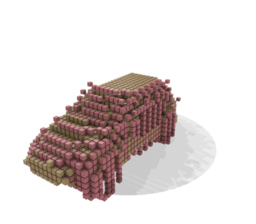
\includegraphics[width=1.75cm,trim={0.5cm 0.75cm 1.5cm 1.5cm},clip]{gfx/experiments_shapenet_kitti/vae_occ+sdf_sup/sb.clean.10.large/binvox_points/00007}
    \end{subfigure}
    \begin{subfigure}[t]{0.1\textwidth}
        \vspace{0px}
        \centering
        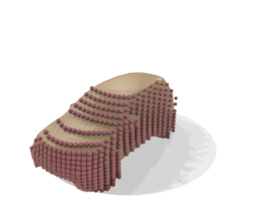
\includegraphics[width=1.75cm,trim={0.5cm 0.75cm 1.5cm 1.5cm},clip]{gfx/experiments_data/clean*/simplified/00007}
    \end{subfigure}
    \begin{subfigure}[t]{0.1\textwidth}
        \vspace{0px}
        \centering
        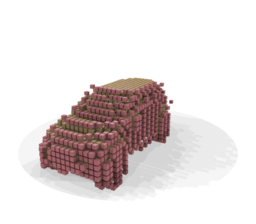
\includegraphics[width=1.75cm,trim={0.5cm 0.75cm 1.5cm 1.5cm},clip]{gfx/experiments_data/clean/voxelized/00007}
    \end{subfigure}\\
    % -------------------------------------------------------------------------------------------------
    % -------------------------------------------------------------------------------------------------
    \begin{subfigure}[t]{0.02\textwidth}
        \vspace{0px}
        \rotatebox{90}{\small\clean\hspace*{0.25cm}}
    \end{subfigure}
    \begin{subfigure}[t]{0.1\textwidth}
        \vspace{0px}
        \centering
        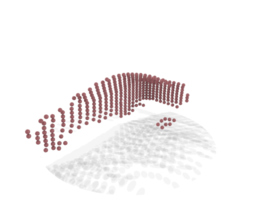
\includegraphics[width=1.75cm,trim={0.5cm 0.75cm 1.5cm 1.5cm},clip]{gfx/experiments_data/clean*/points/00009}
    \end{subfigure}
    \begin{subfigure}[t]{0.1\textwidth}
        \vspace{0px}
        \centering
        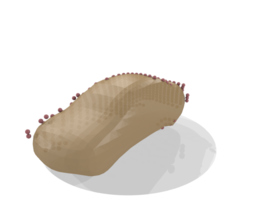
\includegraphics[width=1.75cm,trim={0.5cm 0.75cm 1.5cm 1.5cm},clip]{gfx/experiments_shapenet_kitti/vae_occ+sdf_ml/sb.clean.10.large.const15*/sdf_points/00009}
    \end{subfigure}
    \begin{subfigure}[t]{0.1\textwidth}
        \vspace{0px}
        \centering
        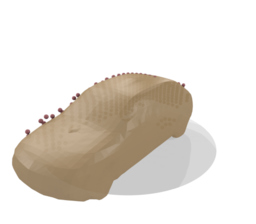
\includegraphics[width=1.75cm,trim={0.5cm 0.75cm 1.5cm 1.5cm},clip]{gfx/experiments_shapenet_kitti/engelmann2016/clean*/sdf_points/00009}
    \end{subfigure}
    \begin{subfigure}[t]{0.1\textwidth}
        \vspace{0px}
        \centering
        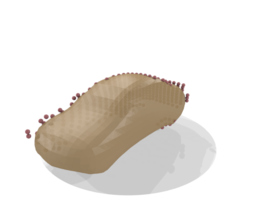
\includegraphics[width=1.75cm,trim={0.5cm 0.75cm 1.5cm 1.5cm},clip]{gfx/experiments_shapenet_kitti/vae_occ+sdf_aml/sb.clean.10.large.const15*/sdf_points/00009}
    \end{subfigure}
    \begin{subfigure}[t]{0.1\textwidth}
        \vspace{0px}
        \centering
        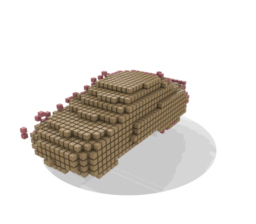
\includegraphics[width=1.75cm,trim={0.5cm 0.75cm 1.5cm 1.5cm},clip]{gfx/experiments_shapenet_kitti/vae_occ+sdf_aml/sb.clean.10.large.const15/binvox_points/00009}
    \end{subfigure}
    \begin{subfigure}[t]{0.1\textwidth}
        \vspace{0px}
        \centering
        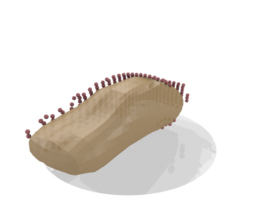
\includegraphics[width=1.75cm,trim={0.5cm 0.75cm 1.5cm 1.5cm},clip]{gfx/experiments_shapenet_kitti/vae_occ+sdf_sup/sb.clean.10.large*/sdf_points/00009}
    \end{subfigure}
    \begin{subfigure}[t]{0.1\textwidth}
        \vspace{0px}
        \centering
        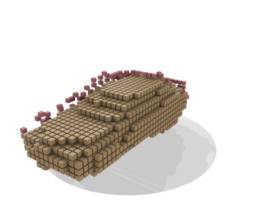
\includegraphics[width=1.75cm,trim={0.5cm 0.75cm 1.5cm 1.5cm},clip]{gfx/experiments_shapenet_kitti/vae_occ+sdf_sup/sb.clean.10.large/binvox_points/00009}
    \end{subfigure}
    \begin{subfigure}[t]{0.1\textwidth}
        \vspace{0px}
        \centering
        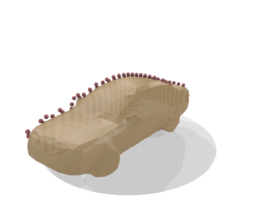
\includegraphics[width=1.75cm,trim={0.5cm 0.75cm 1.5cm 1.5cm},clip]{gfx/experiments_data/clean*/simplified/00009}
    \end{subfigure}
    \begin{subfigure}[t]{0.1\textwidth}
        \vspace{0px}
        \centering
        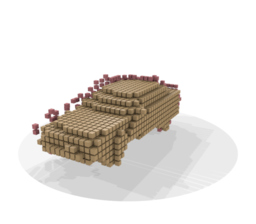
\includegraphics[width=1.75cm,trim={0.5cm 0.75cm 1.5cm 1.5cm},clip]{gfx/experiments_data/clean/voxelized/00009}
    \end{subfigure}
    \hspace*{1cm}{\color{black!25}\rule{0.95\linewidth}{0.5px}}\\[-0.4cm]
    % -------------------------------------------------------------------------------------------------
    % -------------------------------------------------------------------------------------------------
    \begin{subfigure}[t]{0.02\textwidth}
        \vspace{0px}
        \rotatebox{90}{\small\noisy\hspace*{0.2cm}}
    \end{subfigure}
    \begin{subfigure}[t]{0.1\textwidth}
        \vspace{0px}
        \centering
        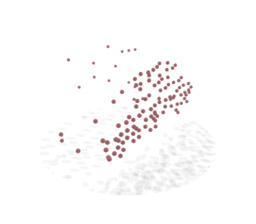
\includegraphics[width=1.75cm,trim={0.5cm 0.75cm 1.5cm 1.5cm},clip]{gfx/experiments_data/noisy*/points/00015}
    \end{subfigure}
    \begin{subfigure}[t]{0.1\textwidth}
        \vspace{0px}
        \centering
        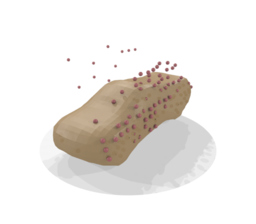
\includegraphics[width=1.75cm,trim={0.5cm 0.75cm 1.5cm 1.5cm},clip]{gfx/experiments_shapenet_kitti/vae_occ+sdf_ml/sb.noisy.10.large.weighted.const50*/sdf_points/00015}
    \end{subfigure}
    \begin{subfigure}[t]{0.1\textwidth}
        \vspace{0px}
        \centering
        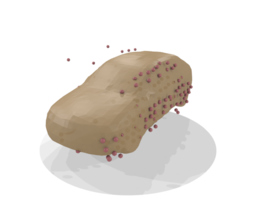
\includegraphics[width=1.75cm,trim={0.5cm 0.75cm 1.5cm 1.5cm},clip]{gfx/experiments_shapenet_kitti/engelmann2016/noisy*/sdf_points/00015}
    \end{subfigure}
    \begin{subfigure}[t]{0.1\textwidth}
        \vspace{0px}
        \centering
        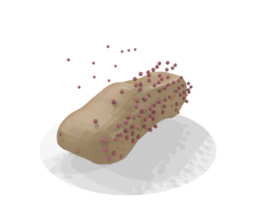
\includegraphics[width=1.75cm,trim={0.5cm 0.75cm 1.5cm 1.5cm},clip]{gfx/experiments_shapenet_kitti/vae_occ+sdf_aml/sb.noisy.10.large.weighted.const50*/sdf_points/00015}
    \end{subfigure}
    \begin{subfigure}[t]{0.1\textwidth}
        \vspace{0px}
        \centering
        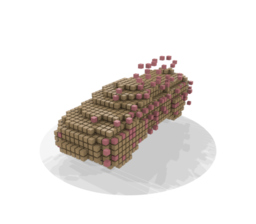
\includegraphics[width=1.75cm,trim={0.5cm 0.75cm 1.5cm 1.5cm},clip]{gfx/experiments_shapenet_kitti/vae_occ+sdf_aml/sb.noisy.10.large.weighted.const50/binvox_points/00015}
    \end{subfigure}
    \begin{subfigure}[t]{0.1\textwidth}
        \vspace{0px}
        \centering
        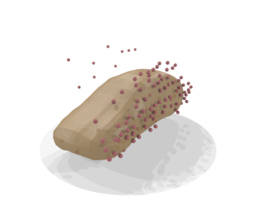
\includegraphics[width=1.75cm,trim={0.5cm 0.75cm 1.5cm 1.5cm},clip]{gfx/experiments_shapenet_kitti/vae_occ+sdf_sup/sb.noisy.10.large*/sdf_points/00015}
    \end{subfigure}
    \begin{subfigure}[t]{0.1\textwidth}
        \vspace{0px}
        \centering
        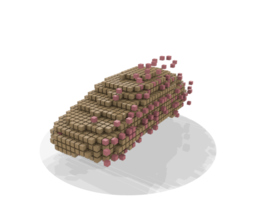
\includegraphics[width=1.75cm,trim={0.5cm 0.75cm 1.5cm 1.5cm},clip]{gfx/experiments_shapenet_kitti/vae_occ+sdf_sup/sb.noisy.10.large/binvox_points/00015}
    \end{subfigure}
    \begin{subfigure}[t]{0.1\textwidth}
        \vspace{0px}
        \centering
        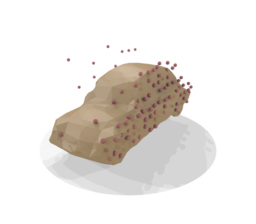
\includegraphics[width=1.75cm,trim={0.5cm 0.75cm 1.5cm 1.5cm},clip]{gfx/experiments_data/noisy*/simplified/00015}
    \end{subfigure}
    \begin{subfigure}[t]{0.1\textwidth}
        \vspace{0px}
        \centering
        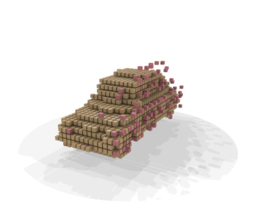
\includegraphics[width=1.75cm,trim={0.5cm 0.75cm 1.5cm 1.5cm},clip]{gfx/experiments_data/noisy/voxelized/00015}
    \end{subfigure}\\
    % -------------------------------------------------------------------------------------------------
    % -------------------------------------------------------------------------------------------------
    \begin{subfigure}[t]{0.02\textwidth}
        \vspace{0px}
        \rotatebox{90}{\small\noisy\hspace*{0.2cm}}
    \end{subfigure}
    \begin{subfigure}[t]{0.1\textwidth}
        \vspace{0px}
        \centering
        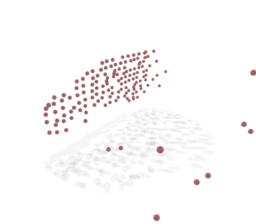
\includegraphics[width=1.75cm,trim={0.5cm 0.75cm 1.5cm 1.5cm},clip]{gfx/experiments_data/noisy*/points/00019}
    \end{subfigure}
    \begin{subfigure}[t]{0.1\textwidth}
        \vspace{0px}
        \centering
        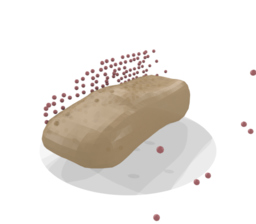
\includegraphics[width=1.75cm,trim={0.5cm 0.75cm 1.5cm 1.5cm},clip]{gfx/experiments_shapenet_kitti/vae_occ+sdf_ml/sb.noisy.10.large.weighted.const50*/sdf_points/00019}
    \end{subfigure}
    \begin{subfigure}[t]{0.1\textwidth}
        \vspace{0px}
        \centering
        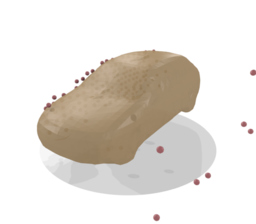
\includegraphics[width=1.75cm,trim={0.5cm 0.75cm 1.5cm 1.5cm},clip]{gfx/experiments_shapenet_kitti/engelmann2016/noisy*/sdf_points/00019}
    \end{subfigure}
    \begin{subfigure}[t]{0.1\textwidth}
        \vspace{0px}
        \centering
        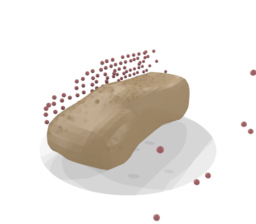
\includegraphics[width=1.75cm,trim={0.5cm 0.75cm 1.5cm 1.5cm},clip]{gfx/experiments_shapenet_kitti/vae_occ+sdf_aml/sb.noisy.10.large.weighted.const50*/sdf_points/00019}
    \end{subfigure}
    \begin{subfigure}[t]{0.1\textwidth}
        \vspace{0px}
        \centering
        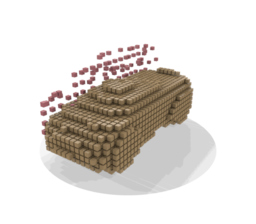
\includegraphics[width=1.75cm,trim={0.5cm 0.75cm 1.5cm 1.5cm},clip]{gfx/experiments_shapenet_kitti/vae_occ+sdf_aml/sb.noisy.10.large.weighted.const50/binvox_points/00019}
    \end{subfigure}
    \begin{subfigure}[t]{0.1\textwidth}
        \vspace{0px}
        \centering
        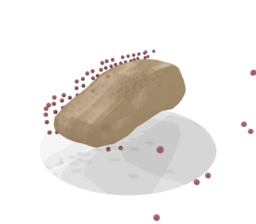
\includegraphics[width=1.75cm,trim={0.5cm 0.75cm 1.5cm 1.5cm},clip]{gfx/experiments_shapenet_kitti/vae_occ+sdf_sup/sb.noisy.10.large*/sdf_points/00019}
    \end{subfigure}
    \begin{subfigure}[t]{0.1\textwidth}
        \vspace{0px}
        \centering
        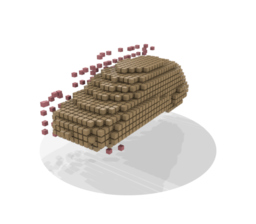
\includegraphics[width=1.75cm,trim={0.5cm 0.75cm 1.5cm 1.5cm},clip]{gfx/experiments_shapenet_kitti/vae_occ+sdf_sup/sb.noisy.10.large/binvox_points/00019}
    \end{subfigure}
    \begin{subfigure}[t]{0.1\textwidth}
        \vspace{0px}
        \centering
        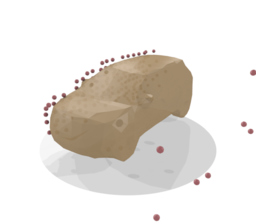
\includegraphics[width=1.75cm,trim={0.5cm 0.75cm 1.5cm 1.5cm},clip]{gfx/experiments_data/noisy*/simplified/00019}
    \end{subfigure}
    \begin{subfigure}[t]{0.1\textwidth}
        \vspace{0px}
        \centering
        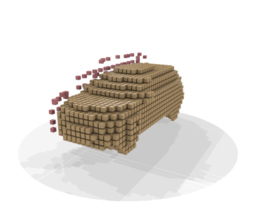
\includegraphics[width=1.75cm,trim={0.5cm 0.75cm 1.5cm 1.5cm},clip]{gfx/experiments_data/noisy/voxelized/00019}
    \end{subfigure}\\
    % -------------------------------------------------------------------------------------------------
    % -------------------------------------------------------------------------------------------------
    \begin{subfigure}[t]{0.02\textwidth}
        \vspace{0px}
        \rotatebox{90}{\small\noisy\hspace*{0.2cm}}
    \end{subfigure}
    \begin{subfigure}[t]{0.1\textwidth}
        \vspace{0px}
        \centering
        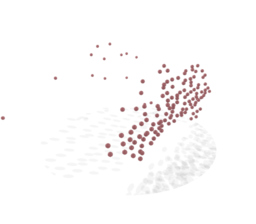
\includegraphics[width=1.75cm,trim={0.5cm 0.75cm 1.5cm 1.5cm},clip]{gfx/experiments_data/noisy*/points/00017}
    \end{subfigure}
    \begin{subfigure}[t]{0.1\textwidth}
        \vspace{0px}
        \centering
        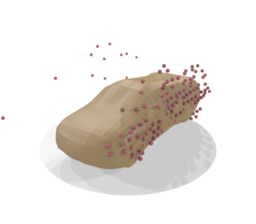
\includegraphics[width=1.75cm,trim={0.5cm 0.75cm 1.5cm 1.5cm},clip]{gfx/experiments_shapenet_kitti/vae_occ+sdf_ml/sb.noisy.10.large.weighted.const50*/sdf_points/00017}
    \end{subfigure}
    \begin{subfigure}[t]{0.1\textwidth}
        \vspace{0px}
        \centering
        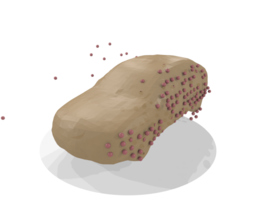
\includegraphics[width=1.75cm,trim={0.5cm 0.75cm 1.5cm 1.5cm},clip]{gfx/experiments_shapenet_kitti/engelmann2016/noisy*/sdf_points/00017}
    \end{subfigure}
    \begin{subfigure}[t]{0.1\textwidth}
        \vspace{0px}
        \centering
        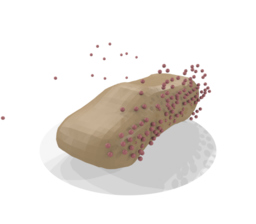
\includegraphics[width=1.75cm,trim={0.5cm 0.75cm 1.5cm 1.5cm},clip]{gfx/experiments_shapenet_kitti/vae_occ+sdf_aml/sb.noisy.10.large.weighted.const50*/sdf_points/00017}
    \end{subfigure}
    \begin{subfigure}[t]{0.1\textwidth}
        \vspace{0px}
        \centering
        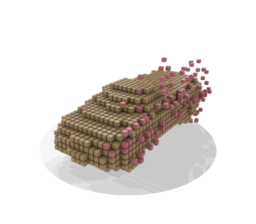
\includegraphics[width=1.75cm,trim={0.5cm 0.75cm 1.5cm 1.5cm},clip]{gfx/experiments_shapenet_kitti/vae_occ+sdf_aml/sb.noisy.10.large.weighted.const50/binvox_points/00017}
    \end{subfigure}
    \begin{subfigure}[t]{0.1\textwidth}
        \vspace{0px}
        \centering
        \includegraphics[width=1.75cm,trim={0.5cm 0.75cm 1.5cm 1.5cm},clip]{gfx/experiments_shapenet_kitti/vae_occ+sdf_sup/sb.noisy.10.large*/sdf_points/00017}
    \end{subfigure}
    \begin{subfigure}[t]{0.1\textwidth}
        \vspace{0px}
        \centering
        \includegraphics[width=1.75cm,trim={0.5cm 0.75cm 1.5cm 1.5cm},clip]{gfx/experiments_shapenet_kitti/vae_occ+sdf_sup/sb.noisy.10.large/binvox_points/00017}
    \end{subfigure}
    \begin{subfigure}[t]{0.1\textwidth}
        \vspace{0px}
        \centering
        \includegraphics[width=1.75cm,trim={0.5cm 0.75cm 1.5cm 1.5cm},clip]{gfx/experiments_data/noisy*/simplified/00017}
    \end{subfigure}
    \begin{subfigure}[t]{0.1\textwidth}
        \vspace{0px}
        \centering
        \includegraphics[width=1.75cm,trim={0.5cm 0.75cm 1.5cm 1.5cm},clip]{gfx/experiments_data/noisy/voxelized/00017}
    \end{subfigure}
    \hspace*{1cm}{\color{black!25}\rule{0.95\linewidth}{0.5px}}\\[-0.4cm]
    % -------------------------------------------------------------------------------------------------
    % -------------------------------------------------------------------------------------------------
    \begin{subfigure}[t]{0.02\textwidth}
        \vspace{0px}
        \rotatebox{90}{\small KITTI\hspace{0.5cm}}
    \end{subfigure}
    \begin{subfigure}[t]{0.1\textwidth}
        \vspace{0px}
        \centering
        \includegraphics[width=1.75cm,trim={0.5cm 0.75cm 1.5cm 1.5cm},clip]{gfx/experiments_data/kitti*/points/00020}
    \end{subfigure}
    \begin{subfigure}[t]{0.1\textwidth}
        \vspace{0px}
        \centering
        \hphantom{\includegraphics[width=1.75cm,trim={0.5cm 0.75cm 1.5cm 1.5cm},clip]{gfx/experiments_shapenet_kitti/engelmann2016/kitti_corrected*/sdf_points/00020}}
    \end{subfigure}
    \begin{subfigure}[t]{0.1\textwidth}
        \vspace{0px}
        \centering
        \includegraphics[width=1.75cm,trim={0.5cm 0.75cm 1.5cm 1.5cm},clip]{gfx/experiments_shapenet_kitti/engelmann2016/kitti_corrected*/sdf_points/00020}
    \end{subfigure}
    \begin{subfigure}[t]{0.1\textwidth}
        \vspace{0px}
        \centering
        \includegraphics[width=1.75cm,trim={0.5cm 0.75cm 1.5cm 1.5cm},clip]{gfx/experiments_shapenet_kitti/vae_occ+sdf_aml/sb.corrected.large.padding.const10*/sdf_points/00020}
    \end{subfigure}
    \begin{subfigure}[t]{0.1\textwidth}
        \vspace{0px}
        \centering
        \includegraphics[width=1.75cm,trim={0.5cm 0.75cm 1.5cm 1.5cm},clip]{gfx/experiments_shapenet_kitti/vae_occ+sdf_aml/sb.corrected.large.padding.const10*/binvox_points/00020}
    \end{subfigure}
    \begin{subfigure}[t]{0.1\textwidth}
        \vspace{0px}
        \centering
        \includegraphics[width=1.75cm,trim={0.5cm 0.75cm 1.5cm 1.5cm},clip]{gfx/experiments_shapenet_kitti/vae_occ+sdf_sup/sb.corrected.large.padding*/sdf_points/00020}
    \end{subfigure}
    \begin{subfigure}[t]{0.1\textwidth}
        \vspace{0px}
        \centering
        \includegraphics[width=1.75cm,trim={0.5cm 0.75cm 1.5cm 1.5cm},clip]{gfx/experiments_shapenet_kitti/vae_occ+sdf_sup/sb.corrected.large.padding*/binvox_points/00020}
    \end{subfigure}
    \begin{subfigure}[t]{0.1\textwidth}
        \vspace{0px}
        \centering
        \includegraphics[width=1.75cm,trim={0.5cm 0.75cm 1.5cm 1.5cm},clip]{gfx/experiments_data/kitti*/points/00020}
    \end{subfigure}
    \begin{subfigure}[t]{0.1\textwidth}
        \vspace{0px}
        \centering
        \includegraphics[width=1.75cm,trim={0.5cm 0.75cm 1.5cm 1.5cm},clip]{gfx/experiments_data/kitti*/gt/00020}
    \end{subfigure}\\
    % -------------------------------------------------------------------------------------------------
    % -------------------------------------------------------------------------------------------------
    \begin{subfigure}[t]{0.02\textwidth}
        \vspace{0px}
        \rotatebox{90}{\small KITTI\hspace{0.5cm}}
    \end{subfigure}
    \begin{subfigure}[t]{0.1\textwidth}
        \vspace{0px}
        \centering
        \includegraphics[width=1.75cm,trim={0.5cm 0.75cm 1.5cm 1.5cm},clip]{gfx/experiments_data/kitti*/points/00008}
    \end{subfigure}
    \begin{subfigure}[t]{0.1\textwidth}
        \vspace{0px}
        \centering
        \hphantom{\includegraphics[width=1.75cm,trim={0.5cm 0.75cm 1.5cm 1.5cm},clip]{gfx/experiments_shapenet_kitti/engelmann2016/kitti_corrected*/sdf_points/00008}}
    \end{subfigure}
    \begin{subfigure}[t]{0.1\textwidth}
        \vspace{0px}
        \centering
        \includegraphics[width=1.75cm,trim={0.5cm 0.75cm 1.5cm 1.5cm},clip]{gfx/experiments_shapenet_kitti/engelmann2016/kitti_corrected*/sdf_points/00008}
    \end{subfigure}
    \begin{subfigure}[t]{0.1\textwidth}
        \vspace{0px}
        \centering
        \includegraphics[width=1.75cm,trim={0.5cm 0.75cm 1.5cm 1.5cm},clip]{gfx/experiments_shapenet_kitti/vae_occ+sdf_aml/sb.corrected.large.padding.const10*/sdf_points/00008}
    \end{subfigure}
    \begin{subfigure}[t]{0.1\textwidth}
        \vspace{0px}
        \centering
        \includegraphics[width=1.75cm,trim={0.5cm 0.75cm 1.5cm 1.5cm},clip]{gfx/experiments_shapenet_kitti/vae_occ+sdf_aml/sb.corrected.large.padding.const10*/binvox_points/00008}
    \end{subfigure}
    \begin{subfigure}[t]{0.1\textwidth}
        \vspace{0px}
        \centering
        \includegraphics[width=1.75cm,trim={0.5cm 0.75cm 1.5cm 1.5cm},clip]{gfx/experiments_shapenet_kitti/vae_occ+sdf_sup/sb.corrected.large.padding*/sdf_points/00008}
    \end{subfigure}
    \begin{subfigure}[t]{0.1\textwidth}
        \vspace{0px}
        \centering
        \includegraphics[width=1.75cm,trim={0.5cm 0.75cm 1.5cm 1.5cm},clip]{gfx/experiments_shapenet_kitti/vae_occ+sdf_sup/sb.corrected.large.padding*/binvox_points/00008}
    \end{subfigure}
    \begin{subfigure}[t]{0.1\textwidth}
        \vspace{0px}
        \centering
        \includegraphics[width=1.75cm,trim={0.5cm 0.75cm 1.5cm 1.5cm},clip]{gfx/experiments_data/kitti*/points/00008}
    \end{subfigure}
    \begin{subfigure}[t]{0.1\textwidth}
        \vspace{0px}
        \centering
        \includegraphics[width=1.75cm,trim={0.5cm 0.75cm 1.5cm 1.5cm},clip]{gfx/experiments_data/kitti*/gt/00008}
    \end{subfigure}\\
    % -------------------------------------------------------------------------------------------------
    % -------------------------------------------------------------------------------------------------
    \begin{subfigure}[t]{0.02\textwidth}
        \vspace{0px}
        \rotatebox{90}{\small KITTI\hspace{0.5cm}}
    \end{subfigure}
    \begin{subfigure}[t]{0.1\textwidth}
        \vspace{0px}
        \centering
        \includegraphics[width=1.75cm,trim={0.5cm 0.75cm 1.5cm 1.5cm},clip]{gfx/experiments_data/kitti*/points/00056}
    \end{subfigure}
    \begin{subfigure}[t]{0.1\textwidth}
        \vspace{0px}
        \centering
        \hphantom{\includegraphics[width=1.75cm,trim={0.5cm 0.75cm 1.5cm 1.5cm},clip]{gfx/experiments_shapenet_kitti/engelmann2016/kitti_corrected*/sdf_points/00056}}
    \end{subfigure}
    \begin{subfigure}[t]{0.1\textwidth}
        \vspace{0px}
        \centering
        \includegraphics[width=1.75cm,trim={0.5cm 0.75cm 1.5cm 1.5cm},clip]{gfx/experiments_shapenet_kitti/engelmann2016/kitti_corrected*/sdf_points/00056}
    \end{subfigure}
    \begin{subfigure}[t]{0.1\textwidth}
        \vspace{0px}
        \centering
        \includegraphics[width=1.75cm,trim={0.5cm 0.75cm 1.5cm 1.5cm},clip]{gfx/experiments_shapenet_kitti/vae_occ+sdf_aml/sb.corrected.large.padding.const10*/sdf_points/00056}
    \end{subfigure}
    \begin{subfigure}[t]{0.1\textwidth}
        \vspace{0px}
        \centering
        \includegraphics[width=1.75cm,trim={0.5cm 0.75cm 1.5cm 1.5cm},clip]{gfx/experiments_shapenet_kitti/vae_occ+sdf_aml/sb.corrected.large.padding.const10*/binvox_points/00056}
    \end{subfigure}
    \begin{subfigure}[t]{0.1\textwidth}
        \vspace{0px}
        \centering
        \includegraphics[width=1.75cm,trim={0.5cm 0.75cm 1.5cm 1.5cm},clip]{gfx/experiments_shapenet_kitti/vae_occ+sdf_sup/sb.corrected.large.padding*/sdf_points/00056}
    \end{subfigure}
    \begin{subfigure}[t]{0.1\textwidth}
        \vspace{0px}
        \centering
        \includegraphics[width=1.75cm,trim={0.5cm 0.75cm 1.5cm 1.5cm},clip]{gfx/experiments_shapenet_kitti/vae_occ+sdf_sup/sb.corrected.large.padding*/binvox_points/00056}
    \end{subfigure}
    \begin{subfigure}[t]{0.1\textwidth}
        \vspace{0px}
        \centering
        \includegraphics[width=1.75cm,trim={0.5cm 0.75cm 1.5cm 1.5cm},clip]{gfx/experiments_data/kitti*/points/00056}
    \end{subfigure}
    \begin{subfigure}[t]{0.1\textwidth}
        \vspace{0px}
        \centering
        \includegraphics[width=1.75cm,trim={0.5cm 0.75cm 1.5cm 1.5cm},clip]{gfx/experiments_data/kitti*/gt/00056}
    \end{subfigure}\\
    % -------------------------------------------------------------------------------------------------
    % -------------------------------------------------------------------------------------------------
    \begin{subfigure}[t]{0.02\textwidth}
        \vspace{0px}
        \rotatebox{90}{\small KITTI\hspace{0.5cm}}
    \end{subfigure}
    \begin{subfigure}[t]{0.1\textwidth}
        \vspace{0px}
        \centering
        \includegraphics[width=1.75cm,trim={0.5cm 0.75cm 1.5cm 1.5cm},clip]{gfx/experiments_data/kitti*/points/00052}
    \end{subfigure}
    \begin{subfigure}[t]{0.1\textwidth}
        \vspace{0px}
        \centering
        \hphantom{\includegraphics[width=1.75cm,trim={0.5cm 0.75cm 1.5cm 1.5cm},clip]{gfx/experiments_shapenet_kitti/engelmann2016/kitti_corrected*/sdf_points/00052}}
    \end{subfigure}
    \begin{subfigure}[t]{0.1\textwidth}
        \vspace{0px}
        \centering
        \includegraphics[width=1.75cm,trim={0.5cm 0.75cm 1.5cm 1.5cm},clip]{gfx/experiments_shapenet_kitti/engelmann2016/kitti_corrected*/sdf_points/00052}
    \end{subfigure}
    \begin{subfigure}[t]{0.1\textwidth}
        \vspace{0px}
        \centering
        \includegraphics[width=1.75cm,trim={0.5cm 0.75cm 1.5cm 1.5cm},clip]{gfx/experiments_shapenet_kitti/vae_occ+sdf_aml/sb.corrected.large.padding.const10*/sdf_points/00052}
    \end{subfigure}
    \begin{subfigure}[t]{0.1\textwidth}
        \vspace{0px}
        \centering
        \includegraphics[width=1.75cm,trim={0.5cm 0.75cm 1.5cm 1.5cm},clip]{gfx/experiments_shapenet_kitti/vae_occ+sdf_aml/sb.corrected.large.padding.const10*/binvox_points/00052}
    \end{subfigure}
    \begin{subfigure}[t]{0.1\textwidth}
        \vspace{0px}
        \centering
        \includegraphics[width=1.75cm,trim={0.5cm 0.75cm 1.5cm 1.5cm},clip]{gfx/experiments_shapenet_kitti/vae_occ+sdf_sup/sb.corrected.large.padding*/sdf_points/00052}
    \end{subfigure}
    \begin{subfigure}[t]{0.1\textwidth}
        \vspace{0px}
        \centering
        \includegraphics[width=1.75cm,trim={0.5cm 0.75cm 1.5cm 1.5cm},clip]{gfx/experiments_shapenet_kitti/vae_occ+sdf_sup/sb.corrected.large.padding*/binvox_points/00052}
    \end{subfigure}
    \begin{subfigure}[t]{0.1\textwidth}
        \vspace{0px}
        \centering
        \includegraphics[width=1.75cm,trim={0.5cm 0.75cm 1.5cm 1.5cm},clip]{gfx/experiments_data/kitti*/points/00052}
    \end{subfigure}
    \begin{subfigure}[t]{0.1\textwidth}
        \vspace{0px}
        \centering
        \includegraphics[width=1.75cm,trim={0.5cm 0.75cm 1.5cm 1.5cm},clip]{gfx/experiments_data/kitti*/gt/00052}
    \end{subfigure}
    \caption{{\bf Additional Qualitative Results.} On \clean and \noisy we present results for \ML, \cite{Engelmann2016GCPR}, \AML and \Sup; as reference, we show the ground truth shapes including observations. On KITTI, we show results for \cite{Engelmann2016GCPR}, \AML and \Sup. As ground truth shapes are not available, we show the accumulated ground truth points instead. In all cases, we show predicted shapes (meshes and occupancy, {\color{rbeige}beige}) and observed points ({\color{rred}red}).}
    \label{fig:appendix-experiments-shapenet-kitti}
\end{figure*}